\section{Modelling Pre-requisites}
\label{sec:modellingprerequisites}
%************************************************
%\section{Method}
%\label{sec:method}
%************************************************

%%%\lipsum[1]
%%\begin{equation}
\label{eq:emc}
e = mc^2
\end{equation}


\subsection{Macroscopic Experiments}
\label{subsec:Macroscopicexperiments}

The first step of the procedure was using a SRSCT (see \cite{RefWorks:142}) to characterize particle flow properties, 
especially the complete yield locus.
With the procedure described in \ref{subsec:srsctexperiment} we
obtained for each of the twelve load conditions three values representative of the bulk behaviour: bulk density ($\rho_b$),
coefficient of internal friction in the pre-shear phase $ (\mu_{psh})$ and
coefficient of internal friction in the shear phase  $ (\mu_{sh})$.\\
Furthermore, in order to recreate the repose angle observed in a pile of the real material, 
we performed angle of repose ($AOR$) tests, as the $AOR$ was the fourth
behaviour value. The complete description can be found in
\ref{subsec:aorexperiment}.
Moreover, we sieved the materials samples to obtain the size distribution of the
particles. Six different sifters have been used.\\

\subsection{Discrete element method}
\label{subsec:dem}
The $DEM$ is based on a relatively elementary idea. 
For each particle i inside the domain it follows the trajectory and calculates the force that particle i exerts on particle j. 
The main forces involved are: gravity, contact forces due to collisions and further interactions such as electrostatic, 
Van der Waals, cohesive forces and fluid-solid interactions in multiphase flows. For the raw material used in this work 
Di Renzo and Di Maio \cite{RefWorks:145} suggested using the non-linear Hertzian model without cohesion for 
the particle-particle and particle-wall contacts. 
This granular model uses the following formula for the contact force between two granular particles (Eq. \ref{eq:forceij}):
\begin{equation}
 F_{ij} = 
\begin{cases}
F_{n,ij} + F_{t,ij} = \left( k_n \delta_{n,ij} + \gamma_n v_{n,ij} \right) + \left( k_t \delta_{t,ij} + \gamma_t v_{t,ij} \right) & \text{if } r < d ,\\
0    & \text{if } r > d ,\\
\end{cases}
 \label{eq:forceij}
\end{equation}

where the subscript n stands for normal and t for tangential. 
Here, $k$ and $\gamma$ are respectively the elastic and damping coefficients, 
while $\delta$ and $v$ the displacement and the velocity, $r$ the distance
between two particles of radii $R_i$ and $R_j$ and $d = R_i + R_j $ is the
contact distance.
Both the normal and the tangential
force comprise two terms, a spring force and a damping force. 
The shear force is a "history" effect that accounts for the tangential displacement 
("tangential overlap") between the particles for the duration of contact. 
The tangential force component is truncated to fulfil 
\begin{equation}
F_{t,ij} \leq \mu_s F_{n,ij},
 \label{eq:force_t}
\end{equation}

where $\mu_s$ is the coefficient of sliding friction, one of the particle based
$DEM$ parameter we investigated. 
An ulterior parameter was the coefficient of rolling friction ($\mu_r$). 
For coarse not round particles is a critical parameter and describes inter-particle 
friction in medium to dense granular flows simulations. It is proportional to the 
torque counteracting the rotation of the particle. The $\mu_r$ parameter enters the 
equations according to the elasto-rolling resistance model presented by Wensrich and 
Katterfeld \cite{RefWorks:87} and Ai et al. \cite{RefWorks:131}, 
based on the work of Jiang et al. \cite{RefWorks:143}. 
The model is called $EPSD2$ in $LIGGGHTS$. This is appropriate for the one way
rolling cases as well as the cycling rolling ones.
The maximum magnitude of rolling resistance torque is (Eq. \ref{eq:trmax}):
\begin{equation}
T_{r~max} = \mu_r R_r |\tilde{F_n}| ~,
 \label{eq:trmax}
\end{equation}

where $R_r$ is the equivalent radius and $F_n$ the normal force.
The $DEM$ parameters for the Young's modulus ($E$) and the coefficient of Poisson ($\nu$) 
have been taken from the literature, see \cite{RefWorks:175} and \cite{RefWorks:176}, 
although we reduced the former to increase the time step, following the indications of Ai et al. \cite{RefWorks:131}. 
The particles radii have been approximated from the experimental measurements. 
The last two particle based $DEM$ parameter we investigated were the particle density 
($\rho_p$) and the coefficient of restitution ($COR$), as defined by Ai. et al. \cite{RefWorks:131}. 
There and in the work Wensrich and Katterfeld \cite{RefWorks:87} further details on the method can be found.
The complete description of the shear cell simulations can be found in \ref{subsec:srsctsimulation}, 
while the AOR simulation is presented in \ref{subsec:aorsimulation}.\\

\subsection{Artificial Neural Networks}
\label{subsec:ann}

An Artificial Neural Network ($NN$) is a powerful modellization technique, 
based on non-linear functions (Haykin \cite{RefWorks:158}). 
In this paper, we first use the $NN$ to fit the $DEM$ numerical simulation data, 
and then to process vast amount of parameters combinations. 
The original idea is directly borrowed from human brain design, with neurons and synapses. 
They map combinations of input data into convenient outputs (fitting). 
There is a variety of types of $NN$, remarkably the Feedforward ($FF$) 
and the Radial basis function ($RBF$). For $FF-NN$, considerable amount 
of traning algorithms are available. The most common are based on backpropagation: 
e.g. Levenberg-Marquardt, Bayesian regulation and scaled conjugate gradient. 
To recognize not linearly separable data the standard linear perceptron $NN$ 
has been modified into \textit{FF Multilayer Perceptron Neural Networks (MLPNN)}. 
Here, each processing units or node (neuron) possesses a nonlinear activation function. 
Together, they are interconnected into layers, also linked together. 
The trustworthiness of the $MLPNN$, with a backpropagation reinforcement learning 
training algorithm (scaled conjugate gradient), has been widely demonstrated in the 
literature, see Haykin \cite{RefWorks:158}. Several scientists 
\cite{RefWorks:161, RefWorks:166, RefWorks:167, RefWorks:168, RefWorks:169, RefWorks:170} 
have operated $NN$ to model materials mechanical properties. 
In fact, $MLPNN$ are built with three different layers. 
%\begin{figure}[!htb] 
\centering 
\includegraphics[width=.96\textwidth]{images/original/18NNscheme} 
\caption{NN scheme}
\label{fig:18NNscheme} 
\end{figure}


% \begin{figure}[htp]
%     \centering
%     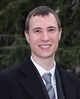
\includegraphics[width=.2\textwidth]{images/vitae/lbenvenuti}
%     \caption{OpenMP, MPI, MPI/OpenMP Hybrid runs of Box in a box testcase on 32
%     cores. The OpenMP-only run suffers from limited memory bandwidth in
%     memory-bound algorithms inside of the Modify section of the code. MPI-only has
%     low averaged runtimes for each section, but a very large Other timing, which
%     hints for a large amount of load-imbalance. Hybrid timings are a bit worse
%     on average, but because of better balancing, processes have lower wait times
%     inside of Other timing.}
% 	\label{fig:boxInBoxComparison}

The input layer has a number of neurons equal to the number of different inputs
of the network, see Fig. \ref{fig:18NNscheme}.
Following the best practice suggested by Vaferi et al. \cite{RefWorks:150} $MLPNN$ have been handled.
Similarly, the best practice also demands to establish the most appropriate number of neurons inside the 
hidden layer of each $NN$. This check has been handled through mean square maximization ($R^2$). 
For each investigated output we chose the number of neurons with the greater
$R^2$.\\
Further, we should question the quality of the NN data, accordingly to the 
Oberkampf et al. \cite{RefWorks:160} method. Haykin \cite{RefWorks:158} 
suggests questioning both the $NN$ training process and the following data generation from given inputs. 
The former is usually challenged when dealing with experimental training data, and frequently 
managed by noise-corrupted patterns calibration. Nevertheless, our training pool
was numerical.
The particles in each of our simulations were created through a random
algorithm, and the training pool was extensive.
For massive training data the effect of noise-corrupted patterns is negligible, see Haykin \cite{RefWorks:158}. 
Instead the latter was a challenging aspect of our work. Once trained, as input for the $NN$ we imposed 
combinations of $DEM$ parameters. 
We tried different methods to generate these combinations. 
Our first attempt was assigning to the investigated variables parameters in even increments 
from the minimum to the maximum values. 
E.g. the $COR$ ranges from 0.5 to 0.9, the first value would be 0.5, the second 0.508163 and so on. 
To increase the generalization, we decided to follow a different approach. 
Random values generators created values in the defined ranges and in the requested 
number for each of the investigated parameter. Then, they were combined and imposed as input.\\
\begin{figure}[!htb] 
\centering 
\includegraphics[width=.96\textwidth]{images/original/18NNscheme} 
\caption{NN scheme}
\label{fig:18NNscheme} 
\end{figure}


% \begin{figure}[htp]
%     \centering
%     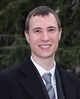
\includegraphics[width=.2\textwidth]{images/vitae/lbenvenuti}
%     \caption{OpenMP, MPI, MPI/OpenMP Hybrid runs of Box in a box testcase on 32
%     cores. The OpenMP-only run suffers from limited memory bandwidth in
%     memory-bound algorithms inside of the Modify section of the code. MPI-only has
%     low averaged runtimes for each section, but a very large Other timing, which
%     hints for a large amount of load-imbalance. Hybrid timings are a bit worse
%     on average, but because of better balancing, processes have lower wait times
%     inside of Other timing.}
% 	\label{fig:boxInBoxComparison}

